\documentclass[11pt]{article}

\usepackage[margin=1in]{geometry}
\usepackage{amsmath,amssymb}
\usepackage{booktabs}
\usepackage{array}
\usepackage{microtype}
\usepackage[hidelinks]{hyperref}
\usepackage{graphicx}
\usepackage{xcolor}

\newcolumntype{L}[1]{>{\raggedright\arraybackslash}p{#1}}

\title{\textbf{PerturbVAE: A Leakage-Aware Benchmark for\\ Single-Cell Perturbation-Response Prediction}}
\author{Brhanu F. Znabu \\ \small University of Nebraska--Lincoln}
\date{June 2026}

\begin{document}
\maketitle

\begin{abstract}
\noindent
PerturbVAE is a conditional variational autoencoder that predicts the
transcriptional response to a genetic perturbation it has never seen, evaluated
under three leakage-controlled held-out splits on two real Perturb-seq datasets
(Norman et al.\ 2019; Replogle et al.\ 2022). The focus of the project is the
evaluation rather than the architecture, which is deliberately small and
standard: how much of the apparent ability to predict perturbation responses
survives when the held-out perturbations are not allowed to be functional
neighbors of the training perturbations, and where a learned model adds value
over a baseline that ignores perturbation identity. The result is mixed and
reported as such. The learned model beats a strong mean-of-training baseline in
one regime, compositional prediction of unseen \emph{double} perturbations
(delta-Pearson $0.748$ vs $0.551$ on Norman), and loses to it on every
single-perturbation split of both datasets. A leakage-free, function-grouped
split changes the measured generalization substantially on a diverse dataset
($-0.27$ Pearson on Norman) and barely at all on a homogeneous one ($-0.02$ on
Replogle), so the leakage gap is real but dataset-dependent. The contribution is
the benchmark design and the honest cross-dataset accounting.
\end{abstract}

\clearpage
\section{Summary of results}

\begin{center}
\begin{tabular}{@{}L{0.46\textwidth} L{0.46\textwidth}@{}}
\toprule
\textbf{Question} & \textbf{Answer} \\
\midrule
Does the cVAE beat a strong baseline anywhere? & Yes, on compositional generalization. Predicting unseen \emph{double} perturbations from singles (Norman), it reaches delta-Pearson $0.748$ vs the mean-of-training baseline's $0.551$ ($+0.20$), and nearly doubles the top-20 DE-gene overlap ($0.34$ vs $0.20$). \\
\addlinespace
Does it beat the baseline on single-perturbation prediction? & No. On every single-perturbation split of both datasets the mean-of-training baseline is higher. The advantage is specific to composition, not single-gene response. \\
\addlinespace
Is there a leakage gap between a random and a leakage-free split? & Yes, but dataset-dependent. Large on Norman (cVAE $-0.27$, baseline $-0.20$); nearly absent on Replogle ($\approx-0.02$). A random-split number can overstate generalization by up to $0.2$ to $0.27$ Pearson. \\
\addlinespace
Is the evaluation honest about scale? & Yes. Two datasets, three split designs, deterministic hashing, a zero-effect control and a strong mean baseline on every split, and DE-gene overlap reported alongside correlation. \\
\bottomrule
\end{tabular}
\end{center}

\clearpage
\section{Motivation}

Perturb-seq couples a CRISPR perturbation to single-cell RNA-seq, so each cell
carries both which gene was hit and what the transcriptome did about it. Models
that predict the response to an unseen perturbation are attractive because the
combinatorial space of perturbations, and especially of \emph{combinations} of
perturbations, is far too large to measure exhaustively. The field reports such
models with delta-correlation against held-out perturbations. Two things make
those numbers easy to over-read, and both are the subject of this project.

\textbf{The baseline is unusually strong.} Most perturbations share a large
common component, a stress / growth-arrest / cell-cycle signature, so predicting
the average training perturbation, ignoring which gene was perturbed, already
correlates respectably with held-out responses. A learned model has to clear that
bar to be useful~\cite{ahlmann2024,kernfeld2023}.

\textbf{The held-out perturbations leak.} A random train/test split routinely
puts a gene's pathway partners or complex members in the training set, so the
model can interpolate to the held-out gene from a functional neighbor it has
already seen. This is the same failure mode as phylogenetic leakage in sequence
models: the test point is not actually novel. The relevant question is how the
model does when \emph{whole functional groups} are withheld. PerturbVAE makes
both unavoidable: a zero-effect control and a mean-of-training baseline on every
split, and a leakage-free, function-grouped split next to the usual random one.

\section{Data}

Both datasets are loaded through the GEARS \texttt{PertData} processed AnnData and
used exactly as distributed (log-normalized expression, conditions in the
\texttt{GENE+ctrl} / \texttt{GENEA+GENEB} / \texttt{ctrl} convention). No synthetic
or simulated data is used anywhere in the results; the only synthetic arrays in
the repository are inside \texttt{tests/}, explicitly as correctness checks.

\begin{center}
\begin{tabular}{@{}lrrrr@{}}
\toprule
Dataset & Cells & Genes & Single conds & Double conds \\
\midrule
Norman 2019 (K562, combinatorial) & 91{,}205 & 5{,}045 & 152 & 131 \\
Replogle 2022 (K562, essential-gene) & 162{,}751 & 5{,}000 & 1{,}092 & 0 \\
\bottomrule
\end{tabular}
\end{center}

Norman is the compositional dataset: it contains genuine two-gene perturbations,
which is what makes split C possible. Replogle is a much larger
single-perturbation screen with no combinations, used to test whether the
single-perturbation findings replicate at roughly seven times the number of
perturbations and on a different experimental design. The prediction target is
the \textbf{pseudobulk delta}: for each condition, the mean expression over its
cells minus the mean over non-targeting control cells.

\section{Evaluation design and contribution}

Three held-out splits, each isolating a different kind of generalization, all
deterministic (BLAKE2b hashing of condition / group keys) so the splits are
identical across machines and runs.

\begin{itemize}
\item \textbf{A, random singles.} A random 80/20 split over single-gene
conditions; the optimistic number matching common practice.
\item \textbf{B, function-grouped singles (leakage-free).} Genes are clustered
into functional groups from their control-cell co-expression signature, and
\emph{entire groups} are held out, so no gene from a held-out group ever appears
in training. Groups are selected smallest-first by deterministic hash until
$\sim$20\% of perturbed genes are withheld. The gap between A and B is the
\textbf{leakage gap}.
\item \textbf{C, combinatorial.} Train on all single perturbations, test on all
\emph{double} perturbations (Norman only). A fixed mean vector structurally
cannot predict an interaction, so this is the split where a learned conditional
model can outperform the baseline.
\end{itemize}

Each held-out perturbation is scored by delta-Pearson, delta-MSE, and the Jaccard
overlap of the top-20 differentially expressed genes; we report the mean across
held-out conditions. To predict a perturbation never seen in training, each gene
is represented by a \textbf{generalizable embedding}, the PCA of its gene-gene
co-expression signature on control cells, defined for every gene. A condition's
embedding is the mean of its perturbed genes' embeddings, which is also what lets
a double perturbation be embedded from two singles in split~C.

\section{Model}

A conditional VAE on the per-cell delta (cell expression minus the control mean):
an encoder $q(z\mid x)$ from the observed delta, a prior $p(z\mid e)$ from the
perturbation embedding $e$, and a decoder $\hat{x}(z,e)$ conditioned on
\emph{both} the latent and the perturbation embedding. Conditioning the decoder
on the perturbation is what lets one trained model produce a different response
for a different (including unseen) perturbation. Because the model is trained on
deltas, the predicted response is read off directly by sampling $z$ from the
perturbation prior and decoding, averaged over draws. It is deliberately small:
64-d latent, 512-d hidden, MSE reconstruction plus KL to the perturbation prior,
$\beta$-annealed over the first third of training, 40 epochs, Adam $10^{-3}$, on a
single L40S / H100. The model is held fixed across all splits.

\section{Baselines}

\textbf{control-mean} predicts zero change for every perturbation (its
delta-Pearson is undefined, so it appears as an MSE floor). \textbf{mean-of-training}
predicts the average training-set delta for every test perturbation, ignoring
which gene was perturbed; this is the strong baseline that captures the shared
stress/growth component dominating most responses.

\section{Results}

\subsection{Per-split performance}

\begin{figure}[h]
\centering
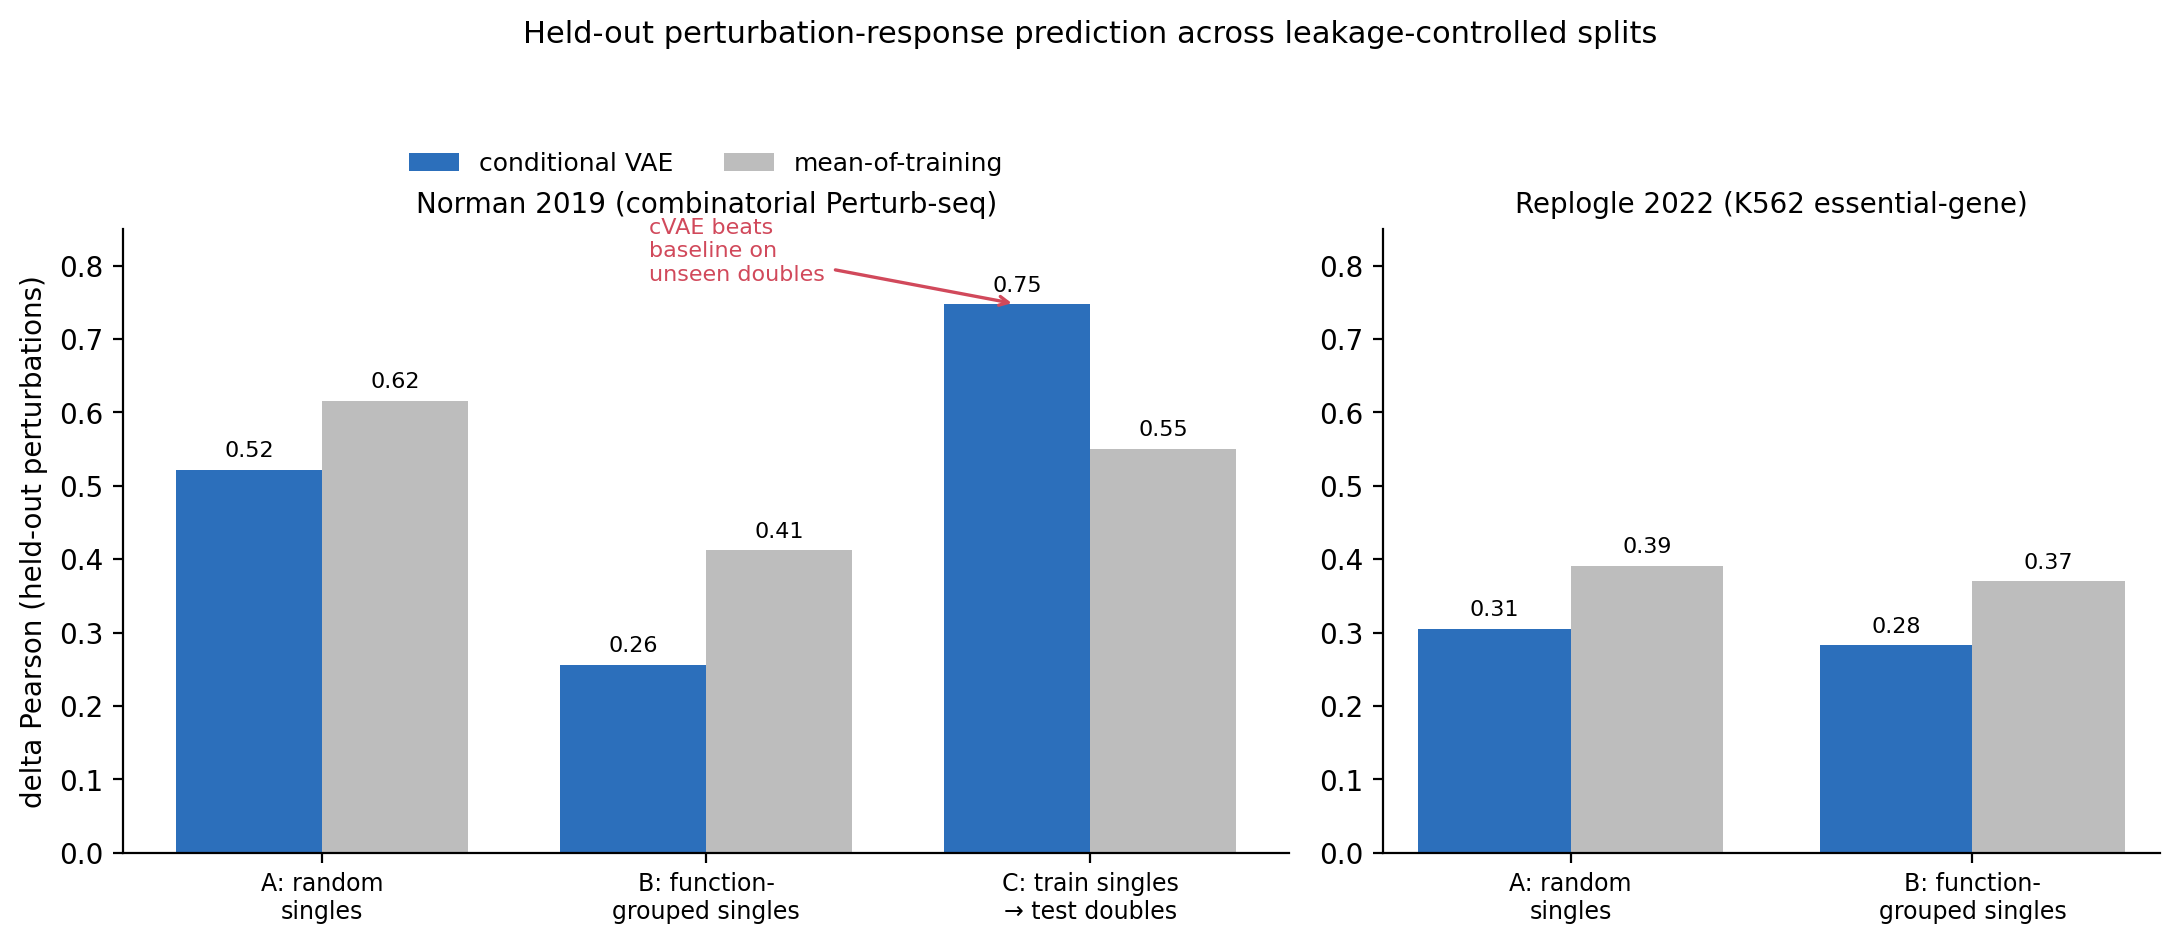
\includegraphics[width=\textwidth]{../figures/fig1_per_split.png}
\caption{Mean delta-Pearson over held-out perturbations, conditional VAE (blue)
vs mean-of-training (grey). Left: Norman, three splits. Right: Replogle, two
splits. The learned model exceeds the strong baseline only on the combinatorial
split.}
\end{figure}

\begin{center}
\begin{tabular}{@{}llrrrrr@{}}
\toprule
Dataset & Split & $n$ test & cVAE $r$ & MoT $r$ & cVAE Jacc. & MoT Jacc. \\
\midrule
Norman & A random & 20 & 0.522 & \textbf{0.616} & 0.243 & 0.266 \\
Norman & B function & 28 & 0.257 & \textbf{0.412} & 0.125 & 0.173 \\
Norman & C combinatorial & 131 & \textbf{0.748} & 0.551 & \textbf{0.341} & 0.199 \\
Replogle & A random & 237 & 0.305 & \textbf{0.391} & 0.084 & 0.072 \\
Replogle & B function & 86 & 0.283 & \textbf{0.370} & 0.082 & 0.076 \\
\bottomrule
\end{tabular}
\end{center}

\textbf{Finding 1: the compositional win.} On Norman's combinatorial split the
cVAE reaches delta-Pearson $0.748$ vs $0.551$ for mean-of-training ($+0.197$), and
the top-20 DE-gene overlap rises from $0.199$ to $0.341$. This is the one regime
where the prediction is genuinely about \emph{interaction}: the joint effect of
two perturbed genes is not the average training delta, and a model that composes
two single-gene embeddings captures structure a fixed vector cannot. This is the
project's positive result.

\textbf{Finding 3: single-perturbation calibration (honest negative).} On every
single-perturbation split of both datasets (A and B, Norman and Replogle), the
mean-of-training baseline is higher than the cVAE. A small VAE trained on a few
hundred to a thousand perturbations does not beat predicting the average response
when the test perturbation is itself a single gene, consistent with the
well-documented difficulty of beating simple baselines on single-perturbation
benchmarks~\cite{ahlmann2024,kernfeld2023}. It is reported here rather than hidden
by quoting only the combinatorial number.

\subsection{The leakage gap}

\begin{figure}[h]
\centering
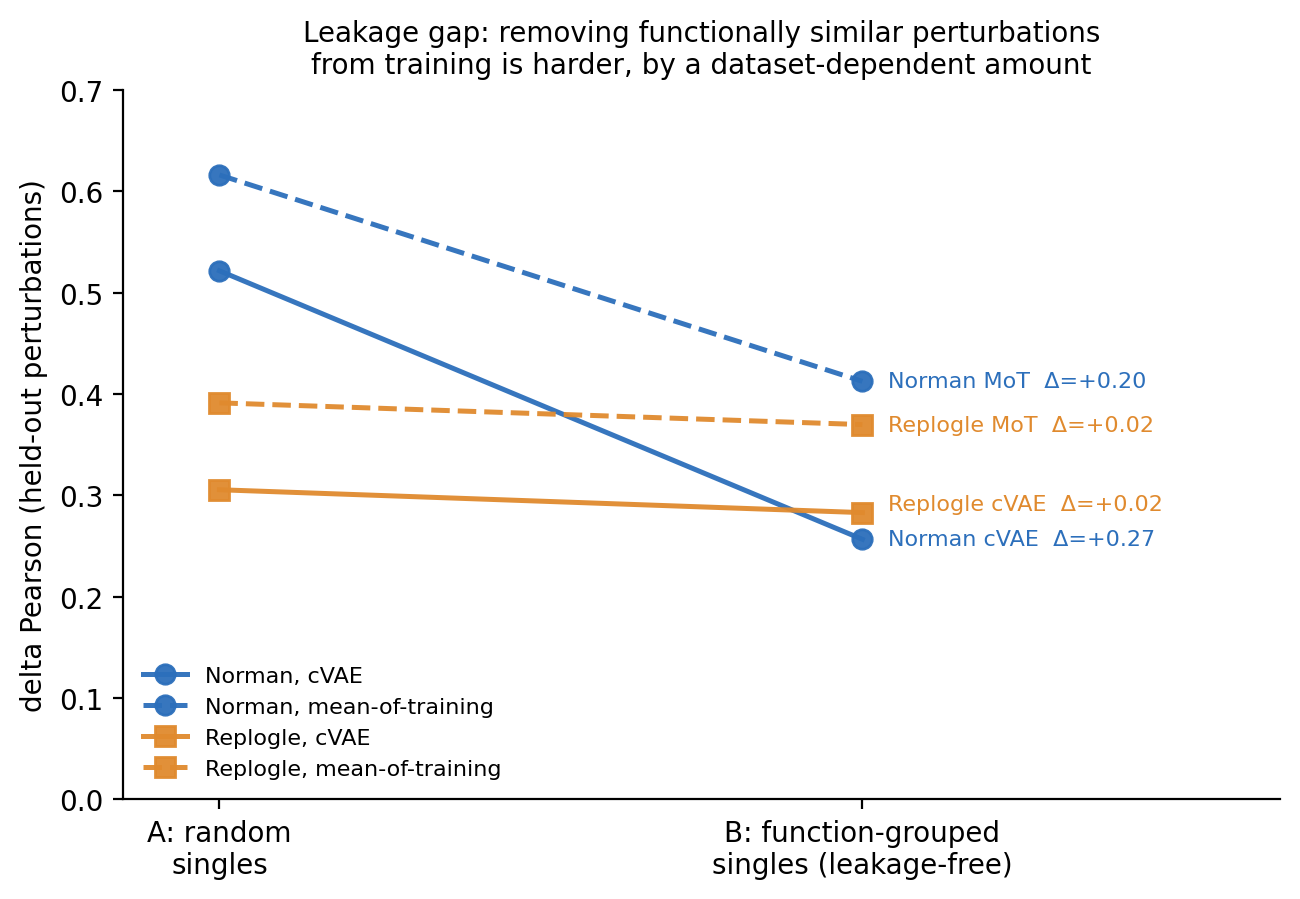
\includegraphics[width=0.82\textwidth]{../figures/fig2_leakage.png}
\caption{Delta-Pearson on the random split (A) vs the leakage-free
function-grouped split (B). The slope is the leakage gap: large on Norman and
almost flat on Replogle, for both the learned model and the baseline.}
\end{figure}

\begin{center}
\begin{tabular}{@{}llrrr@{}}
\toprule
Dataset & Method & A random & B function & gap (A$-$B) \\
\midrule
Norman & cVAE & 0.522 & 0.257 & \textbf{0.265} \\
Norman & mean-of-training & 0.616 & 0.412 & \textbf{0.204} \\
Replogle & cVAE & 0.305 & 0.283 & 0.023 \\
Replogle & mean-of-training & 0.391 & 0.370 & 0.021 \\
\bottomrule
\end{tabular}
\end{center}

\textbf{Finding 2: the leakage gap is real but dataset-dependent.} On Norman,
withholding whole functional groups instead of random genes drops delta-Pearson
by $0.265$ for the cVAE and $0.204$ even for the mean-of-training baseline: a
fifth to a quarter of the apparent random-split performance was interpolation
between functionally similar perturbations, and some of it disappears even for a
model that never looks at gene identity, because random splits also leak through
which conditions land in the test mean. On Replogle the same procedure moves the
number by only $\sim$0.02. The reason is informative rather than contradictory:
Replogle is a 1{,}092-gene essential-gene screen whose responses are dominated by
a single shared growth-arrest signature, so per-perturbation deltas are
relatively homogeneous, the mean baseline is already near the ceiling, and
removing functional neighbors barely changes what is predictable. The leakage gap
is therefore not a universal constant; its size tracks how much
\emph{perturbation-specific} structure a dataset contains. The practical
consequence stands: on a diverse perturbation set a random-split number can
overstate leakage-free generalization by $0.2$ to $0.27$ Pearson, and a
leakage-free split is necessary to know which.

\section{What this shows, and what it does not}

It shows: (i) a learned conditional model can beat a strong, identity-blind
baseline specifically on compositional prediction of unseen perturbation
combinations; (ii) on single-perturbation prediction that same model does not beat
the baseline at this scale; (iii) a leakage-free, function-grouped split changes
measured generalization substantially on a diverse dataset and barely at all on a
homogeneous one. Together these calibrate \emph{when} perturbation-response
prediction is hard and \emph{where} a learned model helps.

It does not show that this particular cVAE is a competitive perturbation model.
The architecture is intentionally small and untuned; larger conditional models
(GEARS, scGPT-style, CPA) would likely raise all of these numbers. The functional
groups are derived from co-expression rather than curated pathway/complex
annotations, a reproducible but coarse proxy for a functional neighbor. And the
evaluation is pseudobulk delta-correlation, which rewards getting the dominant
direction right and is forgiving about the tails. The contribution is the
benchmark design and the honest cross-dataset accounting, not a state-of-the-art
model.

\section{Reproducibility}

Every number is produced by the scripts in the repository from the public
datasets with deterministic splits:

\begin{verbatim}
python src/scripts/run_baselines.py --h5ad data/norman/perturb_processed.h5ad \
    --out results/baselines_norman.json
python src/scripts/train.py --h5ad data/norman/perturb_processed.h5ad \
    --out results/cvae_norman_delta.json --epochs 40
# repeat both with data/replogle_k562_essential/perturb_processed.h5ad
python src/scripts/make_figures.py
\end{verbatim}

\texttt{tests/test\_smoke.py} checks the splits, metrics, baselines, and model on
small synthetic arrays. These are correctness tests, explicitly labeled as such,
not part of any reported result.

\clearpage
\begin{thebibliography}{9}
\bibitem{norman2019} Norman, T.M., Horlbeck, M.A., Replogle, J.M., et al. Exploring genetic interaction manifolds constructed from rich single-cell phenotypes. \emph{Science} 365(6455):786--793, 2019.
\bibitem{replogle2022} Replogle, J.M., Saunders, R.A., Pogson, A.N., et al. Mapping information-rich genotype--phenotype landscapes with genome-scale Perturb-seq. \emph{Cell} 185(14):2559--2575, 2022.
\bibitem{gears2024} Roohani, Y., Huang, K., Leskovec, J. Predicting transcriptional outcomes of novel multigene perturbations with GEARS. \emph{Nature Biotechnology} 42:927--935, 2024.
\bibitem{cpa2023} Lotfollahi, M., Klimovskaia Susmelj, A., De Donno, C., et al. Predicting cellular responses to complex perturbations in high-throughput screens (CPA). \emph{Molecular Systems Biology} 19(6):e11517, 2023.
\bibitem{ahlmann2024} Ahlmann-Eltze, C., Huber, W., Anders, S. Deep-learning-based gene perturbation effect prediction does not yet outperform simple linear baselines. \emph{Nature Methods} 22:1657--1661, 2025.
\bibitem{kernfeld2023} Kernfeld, E., Yang, Y., Weinstock, J.S., Battle, A., Cahan, P. A systematic comparison of computational methods for expression forecasting. \emph{bioRxiv} 2023.07.28.551039, 2023.
\end{thebibliography}

\end{document}
